%=============================--A--=============================%
\subsection{Módulo 2 $\pmb \mapsto$ Recuperaç\~ao da componente mono $(L + R)$}
\label{subsec:mod2}

%\iffalse
\begin{figure}[H]
    \centering
    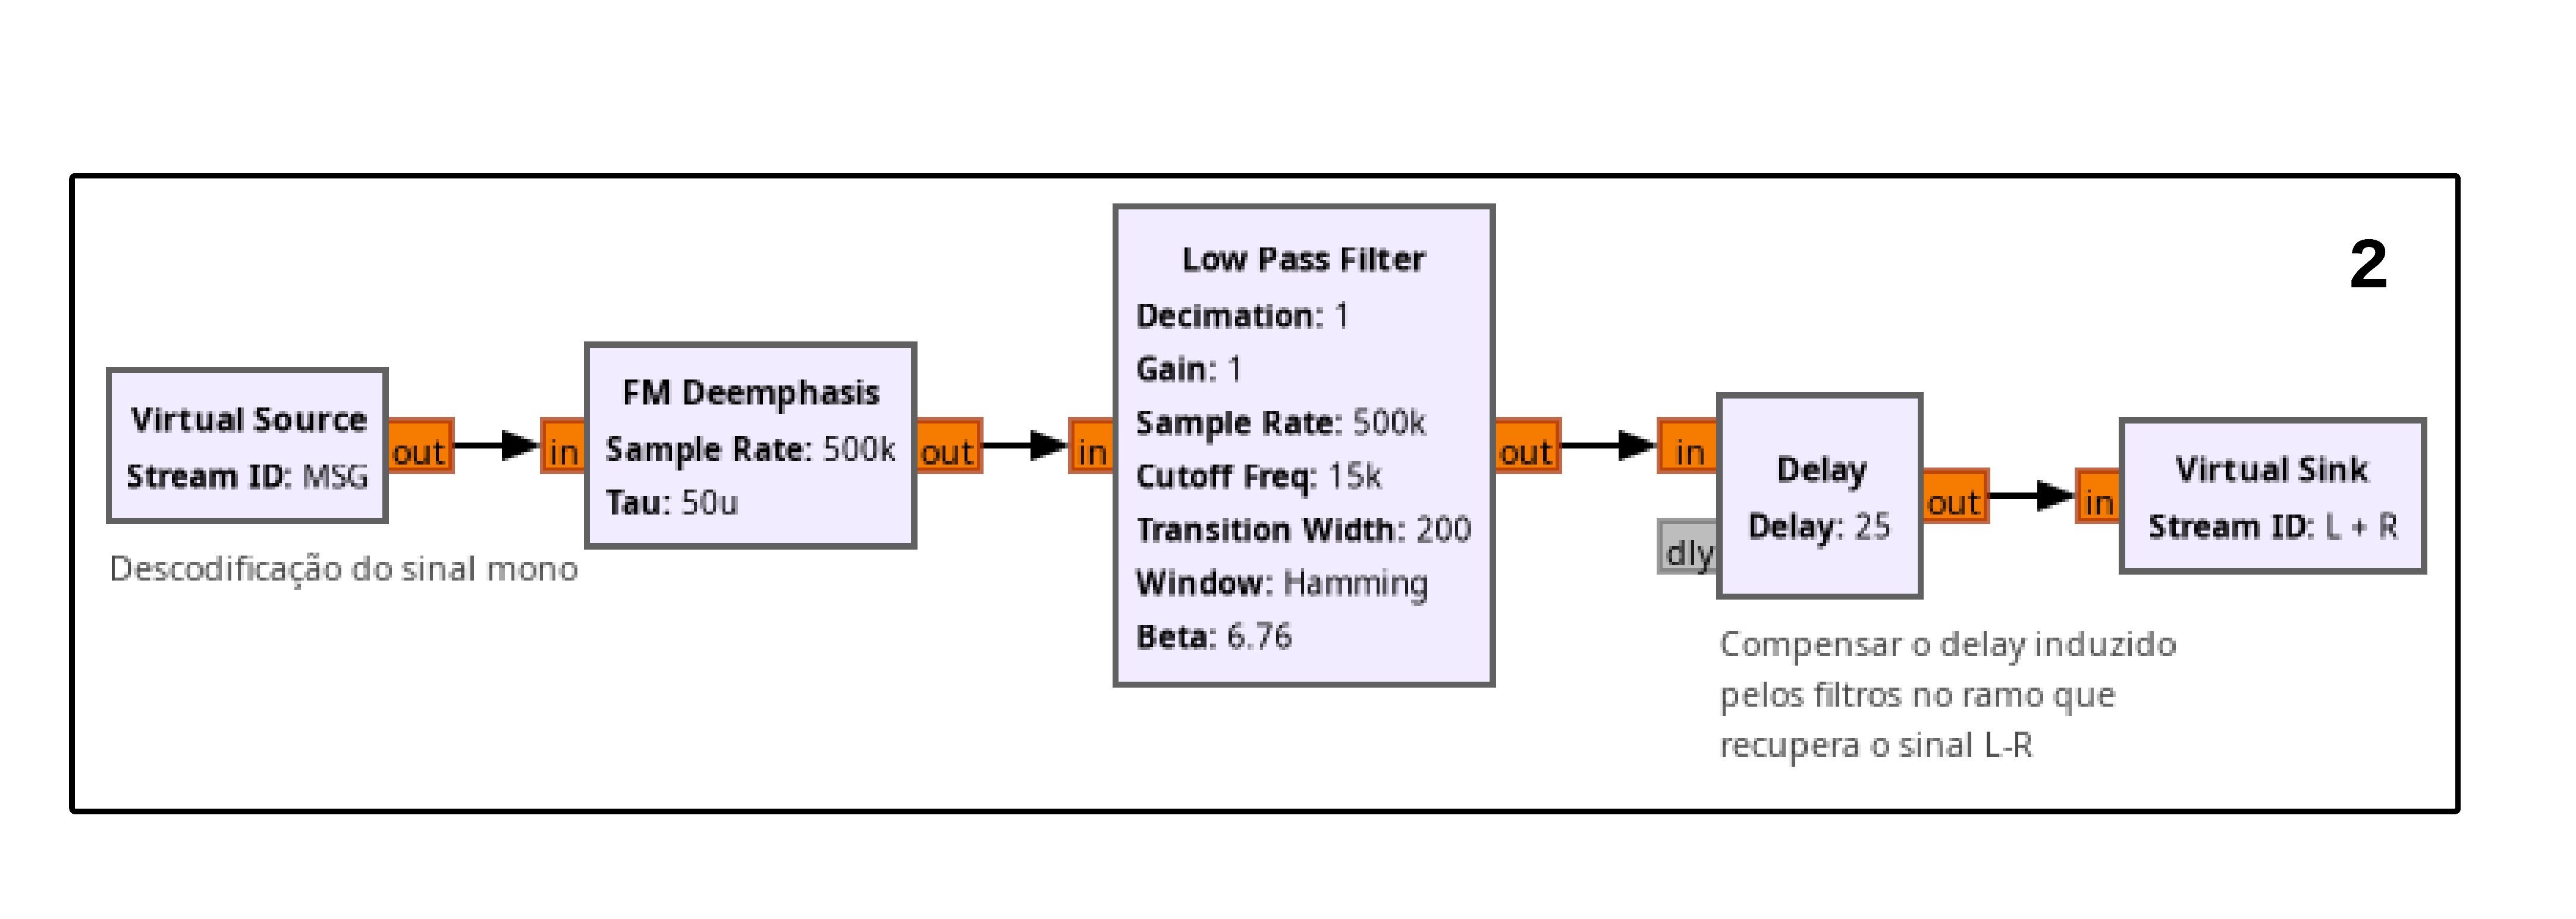
\includegraphics[width = 0.65\linewidth]{img/mods/modulo2.png}
    \caption{Recuperação da componente monofónica da mensagem.}
    \label{fig:modulo2}
\end{figure}
%\fi

De forma sucinta, o \hyperref[subsec:mod2]{módulo 2} recupera o sinal mono ($L+R$), com as correções mencionadas na secção anterior \hyperref[sec:peculiaridades]{(Peculiaridades)}, simplesmente com a aplicação de um filtro passa-baixo com $f_c = 15$ kHz, dado o formato espectral da mensagem multiplexada já abordado na introdução \hyperref[fig:stereo_spectrum]{(Fig. 1)}. 